% Chapter Template

\chapter{Descripteurs d'Images \&  Mesures de Similarité} % Main chapter title

\label{ChapterX} % Change X to a consecutive number; for referencing this chapter elsewhere, use \ref{ChapterX}

%----------------------------------------------------------------------------------------
%	SECTION 1
%----------------------------------------------------------------------------------------

\section{Introduction}
Aujourd’hui avec le développement des systèmes multimédias et le recul de l’écrit, nous utilisons de plus en plus le contenu visuel comme support de communication dans différents domaines. En effet l’image et la vidéo numérique sont partie intégrante de tels systèmes par la
densité et la richesse de leur contenu. La même image peut présenter plusieurs significations à différents niveaux : analyse, description, reconnaissance et interprétation.

La recherche d’information couvre le traitement de documents numériques impliquant la structure, l’analyse, le stockage et l’organisation des données. Dans le passé, le terme recherche d’information était lié au concept de l’information textuelle. Actuellement « RI »est associé à tout type d’information, textuelle, visuelle ou autre. Cependant dû aux limitations des méthodes textuelles, le développement des méthodes basées sur le contenu visuel est devenu primordial. Ceci explique l’activité de recherche intense consacrée au système CBIR ces dernières années. Le « RIC » est souvent confronté au problème de pertinence de la
recherche, et au temps de recherche. L’objectif de n’importe quel système CBIR est de satisfaire la requête d’un utilisateur par la
pertinence des résultats. Comme l’accès à un document via sa pure sémantique est impossible, les systèmes CBIR traditionnels s’appuient sur un paradigme de représentation de bas niveau du contenu de l’image, par la couleur, la texture, la forme, etc.…, et d’autres par une
combinaison de celles-ci. La recherche d’images se fait ainsi par comparaison des descripteurs.

L’analyse et la représentation du contenu des données sources mises sous forme de vecteur caractéristique. L’information obtenue dans cette étape est une sorte de résumé des images de la base (segmentation en régions, couleur, texture, relations spatiales,…). La transformation
est généralement gourmande en temps de calcul.

Dans la suite de ce chapitre, nous présentons les différents attributs utilisés dans les systèmes de recherche d’image par contenu et ensuite les mesures de similarité entre les images après la définition de leurs descripteurs.




%----------------------------------------------------------------------------------------
%	SECTION 2
%----------------------------------------------------------------------------------------

\section{Descripteurs d’image}

%----------------------------------------------------------------------------------------
%	SUBSECTION 1
%----------------------------------------------------------------------------------------
\subsection{Descripteur de la couleur}
La couleur est l’information visuelle la plus utilisée dans les systèmes de recherche par le contenu. Ces valeurs tridimensionnelles font que son potentiel discriminatoire soit supérieur à la valeur en niveaux de gris des images. Mais la caractérisation de la couleur dans une image est une opération extrêmement complexe.

En effet, cette donnée varie considérablement avec l’orientation des surfaces, le point de vue de la caméra et l’illumination (positions et longueur d’onde des sources lumineuses). En outre, la perception de la couleur par l'être humain est un processus complexe et subjectif.

Chaque pixel d'une image numérique est constitué d'un élément de couleur. Dans une image en niveaux de gris, cette couleur varie généralement de 0 à 255, où 0 est noir, 255 est blanc, et les valeurs entre les deux sont les suivantes différentes nuances de gris, du noir au blanc. Dans une image couleur, disons avec une résolution couleur 24 bits (ce qui signifie que 24 bits sont utilisés pour les informations de couleur pour chaque pixel), une partie (souvent paire) des 24 bits est affectée à chacun des trois composants de couleur dans l’image. L'espace colorimétrique le plus couramment utilisé est RVB signifie Rouge-Vert-Bleu (RGB: ReedGreen-Blue). L'espace de couleur est défini comme un modèle pour représenter la couleur en termes de valeurs d'intensité RVB, et dans cet exemple l'image couleur 24 bits, 8 bits sont utilisées pour représenter chacun des composants. Dans cet exemple, les composantes de couleur permettent de représenter $(2 ^ 8) ^ 3$ couleurs différentes, ce qui est difficile de les
distinguer par l'oeil humain.

\begin{figure}[H]
	\label{fig:imageRVB}
	\centering
	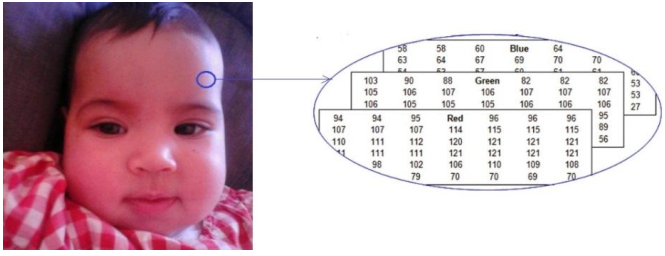
\includegraphics[width=0.65\textwidth]{Figures/imageRVB} % Include the image .png
	
	\caption{Image couleur dans l’espace RVB.}
	
\end{figure}

\begin{figure}[H]
	\label{fig:tableRVB}
	\centering
	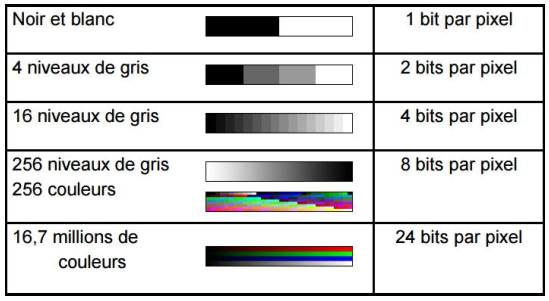
\includegraphics[width=0.65\textwidth]{Figures/tableRVB} % Include the image .png
	
	\caption{Représentation des pixels en fonction de nombre des bits.}
	
\end{figure}

La couleur est devenue un attribut largement utilisé dans les systèmes opérationnels de recherche d'images par le contenu. Elle facilite l'identification et l'extraction d'un objet dans une scène [Zavi01]. Il semble que son efficacité à ce stade soit liée au fait que l'être humain peut distinguer des milliers de couleurs et seulement 24 niveaux de gris [Gonz02].

\subsubsection{L'histogramme}
La plus grande majorité des systèmes de recherche d'images par le contenu se base sur la description des couleurs composant les images. De nombreux travaux ont vu le jour quant à l'utilisation de la couleur pour la recherche d’images par le contenu. L’approche la plus courante dans la littérature est d'indexer la couleur par l'utilisation d'histogrammes de couleurs [Swain91] L'histogramme des couleurs exprime la distribution statistique de celles-ci dans l'image.

Ce type d'histogramme est calculé typiquement sur un espace caractéristique quantifié. Chaque valeur de caractère dans l'histogramme représente donc un rang de couleur dans la
palette. 

L'histogramme a été introduit pour la première fois en RIC par [Swain 91], depuis il est très utilisé à cause de sa simplicité de calcul, son invariante aux changements d'échelle et aux transformations géométriques.\\

\begin{figure}[H]
	\label{fig:hist}
	\centering
	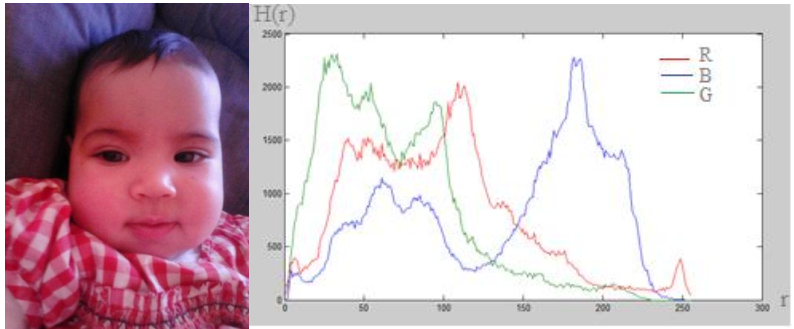
\includegraphics[width=0.65\textwidth]{Figures/hist} % Include the image .png
	\caption{Exemple d’histogramme d’une image couleur.}
\end{figure}

Les inconvénients majeurs de l'histogramme sont:
\begin{itemize}
	\item La perte de toute information spatiale dont la texture ou la forme. Par exemple un histogramme d'un tapis rouge peut être très proche de celui d'une porte rouge ou d'une voiture rouge.
	
	\item Ils sont de grandes tailles, donc par conséquent il est difficile de créer une indexation rapide et efficace en les utilisant tels qu'ils sont. 
	
	\item Ils sont sensibles à de petits changements de luminosité, ce qui est problématique pour comparer des images similaires, mais acquises dans des conditions différentes. 
	
	\item Ils sont inutilisables pour la comparaison partielle des images (objet particulier dans une image), puisque calculés globalement sur toute l’image.
	
\end{itemize}
   Des méthodes alternatives ont été proposées pour augmenter l'efficacité de l'histogramme. Nous citons quelques-unes : 
\begin{itemize}
	\item les moments de la couleur [Stricker 94], [Ravishankar 99],
	\item les constantes de couleur [Flickner 95], [Worring 01],
	\item la signature couleur [Kender 98], 
	\item les blobs [Chang 97] et le vecteur cohérent de couleur [Pass 97].\\
\end{itemize}

Une nouvelle technique à base d'histogrammes locaux de couleurs a été proposée par Wang [Wang 01]. Cette technique est insensible à la rotation. Son principe consiste à diviser une image en un ensemble de blocs égaux et calcule leur histogramme de couleurs. Ainsi elle utilise un graphe biparti pour calculer la distance ayant le coût minimal entre deux images. Enfin chaque bloc de l'image requête est comparé à tous les blocs des images de la base afin de retrouver les images similaires.\\

De point de vue de la recherche CBIR, Alaoui [Alao11] a présenté deux nouveaux descripteurs : le premier descripteur est l’entropie de distribution de couleur « CDE » qui introduit l'entropie pour décrire l'information spatiale des couleurs. Le deuxième descripteur est l’entropie hybride de couleur « CHE » qui introduit une description spatiale à caractère multi-résolution d'images couleurs. Les résultats expérimentaux montrent qu'un système d'indexation CBIR basé sur les descripteurs « CDE » et « CHE » est plus performant que les systèmes CBIR traditionnels basée sur les histogrammes locaux.\\

\subsubsection{Les moments de couleur}
Les moments de couleur on été utilisés dans plusieurs systèmes de recherche d’images par le contenu tel que QBIC, mathématiquement les trois premiers moments sont définis par :
\begin{figure}[H]
	\label{fig:moments}
	\centering
	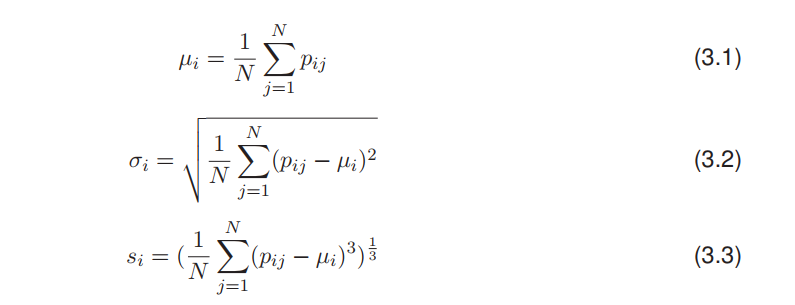
\includegraphics[width=0.65\textwidth]{Figures/moments} % Include the image .png
	\caption{Moments}
	
\end{figure}

Les moments de couleur est une représentation compacte comparée aux autres descripteurs de couleur. Car seulement 9 valeurs (3 pour chaque composante chromatique) sont utilisées pour représenter le contenu d’une image. Pour cette raison ils peuvent diminuer le pouvoir de discrimination (description). 

\subsubsection{Conclusion}
L'information relative aux couleurs est particulièrement importante dans la caractérisation d’une image. Plusieurs études ont été menées pour trouver un critère de choix des descripteurs de couleurs pour l'indexation des images, mais aucune n'a abouti. Ceci peut s’expliquer par le manque de subjectivité de cette information, les descripteurs couleur ne suffisent pas à indexer efficacement une image, ni à la chercher.

Dans plusieurs domaines d’application, l’utilisation de descripteurs résumant l’information globale d’images couleurs, tels que le descripteur des histogrammes locaux de couleurs des images entières, n’offre pas toujours des résultats satisfaisants. Globalement, l’histogramme couleur reste le descripteur le plus utilisé. Bien qu’il ne contienne qu’une information partielle en raison de l’absence d’indication sur les caractéristiques spatiales, l’histogramme garde un fort pouvoir de description, ce qui explique sa grande utilisation.

\begin{figure}[H]
	\label{fig:samehist}
	\centering
	
\includegraphics[width=0.65\textwidth]{Figures/sameHist} % Include the image .png
	\caption{Deux images différentes de même histogramme.}
	
\end{figure}

%----------------------------------------------------------------------------------------
%	SUBSECTION 2
%----------------------------------------------------------------------------------------
\subsection{Descripteur de la texture}
 
Dans [Tuceryan 98], l’auteur présente 4 familles d'outils de caractérisation de la texture. On distingue parmi elles les méthodes statistiques, les méthodes géométriques, les méthodes à base de modèles probabilistes et les méthodes fréquentielles. En utilisant des filtres prédéfinis, la méthode de [Laws 80] utilise des convolutions spatiales pour construire 25 versions d’une image texturée, chaque version décrit une caractéristique précise de l’image.\\


Au même titre que la couleur, l'identification de la texture est une partie importante du système visuel humain, c'est un arrangement spatial de pixels, habituellement dans des modèles visuels homogènes que ni la couleur ni l'intensité moyenne ne décrivent suffisamment. La modélisation et la description des textures sont un problème difficile. La texture est une caractéristique intuitive facile à reconnaître mais difficile à définir.

D’après [7], une définition formelle de la texture est quasiment impossible.

\begin{description}
	\item[Définition:] 	
	D’une manière générale, la texture dans une image peut être définie comme un arrangement spatial de couleurs ou d'intensités dans une région de cette image [Linda 01]. Elles peuvent consister en un placement structuré d’éléments mais peuvent aussi n’avoir aucun élément répétitif.
\end{description}


\begin{figure}[H]
	\label{fig:textures}
	\centering
	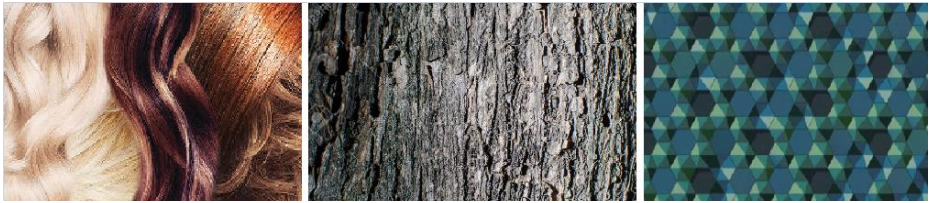
\includegraphics[width=0.65\textwidth]{Figures/textures} % Include the image .png
	
	\caption{Des textures différentes.}
	
\end{figure}

De nombreuses définitions ont été proposées, mais aucune ne convient parfaitement aux différents types de textures rencontrées. Dans une définition couramment citée [36], la texture est présentée comme une structure disposant de certaines propriétés spatiales homogènes et invariantes par translation. Cette définition stipule que la texture donne la même impression à l'observateur quelle que soit la position spatiale de la fenêtre à travers laquelle il observe cette texture. Par contre l’échelle d’observation doit être précisée. On peut le faire par exemple en précisant la taille de la fenêtre d’observation.\\

La notion de texture est liée à trois concepts principaux:
\begin{enumerate}
	\item un certain ordre local qui se répète dans une région de taille assez grande,
	
	\item cet ordre est défini par un arrangement structuré de ses constituants élémentaires,
	
	\item ces constituants élémentaires représentent des entités uniformes qui se caractérisent par des dimensions semblables dans toute la région considérée.\\ 
	
\end{enumerate}

Il existe un grand nombre de textures. On peut les séparer en deux classes:
\begin{itemize}
	\item Les textures
	structurées (macrotextures): constituée par la répétition d’une primitive à intervalle régulier. On peut différencier dans cette classe les textures parfaitement périodiques (carrelage, damier, ...etc.), les textures dont la primitives subit des déformations ou des changements d'orientation (mur de briques, grains de café, ...etc.).
	
	\item Les textures aléatoires (microtextures): se distinguent en général par un aspect plus fin (sable, herbe, ...etc.). Contrairement aux textures de type structurel, les textures aléatoires ne comportent ni primitive isolable, ni fréquence de répétition. On ne peut donc pas extraire de ces textures une primitive qui se répète dans l’image mais plutôt un vecteur de paramètres statistiques homogènes à chaque texture.
\end{itemize}

Dans tous les cas, ces objectifs nécessitent l'extraction d'un ou de plusieurs paramètres caractéristiques de cette texture. Nous désignerons ces paramètres sous le terme d’attributs texturaux (textural features) et l’ensemble qu’ils constituent sous le terme de descripteur de texture.

Certains de ces paramètres correspondent à une propriété visuelle de la texture (comme la directionnalité ou la rugosité). D'autres correspondent à des propriétés purement mathématiques auxquelles il est difficile d'associer une qualification perceptive.

Un recensement ainsi qu'une classification des termes de description des textures employés par les principaux auteurs pourront être trouvés dans [38] et [39].

Il a été prouvé dans la littérature que l'analyse de descripteurs de texture est efficace pour de nombreuses applications, y compris la vision artificielle, la segmentation d'images médicales, la cartographie urbaine, l'analyse d'images satellitaires, la télé-détection.\\

La texture représente également un descripteur bas niveau efficace utilisé dans le cadre de l'indexation et la recherche par le contenu. Les attributs texturaux peuvent être obtenus à partir d’un ensemble assez vaste de différentes théories mathématiques, nous citons notamment :

\subsubsection{Les matrices de co-occurrences (Mesures de Haralick)}

 En 1973, Haralick a proposé une méthode en se basant sur la matrice de co-occurrence de niveaux de gris [Haralick 73], elle est probablement une méthode classiques et la plus célèbre pour l'analyser de la texture.
 
 La texture d’une image peut être interprétée comme la régularité d’apparition de couples de niveaux de gris selon une distance (pas $k=1, 2, 3, ...etc$) donnée dans l’image. La matrice de co-occurrences contient les fréquences spatiales relatives d’apparition des niveaux
 de gris selon quatre directions: $\theta = 0◦$,  $\theta =  \frac{\pi}{4} = 45◦$,  $\theta =  \frac{\pi}{2} = 90◦$,  $\theta =  3 \times \frac{\pi}{4} = 135◦$. Une matrice de co-occurrences est définie au moyen d’une relation entre deux pixels .\\

\begin{description}
	\item[Définition] La matrice de coocurrence $P_{d,\theta}=(P_{d,\theta}(i, j))_{1\leq i,j \leq Ng}$ est une matrice carrée de taille $Ng \times Ng$. Avec:
	\begin{itemize}
		\item Ng étant le nombre de niveaux de gris de l'image (256x256). Les indices de la matrice de co-occurrences sont
		donc les niveaux de gris de la texture étudiée.
		\item On réduit souvent a des tailles 8x8, 16x16 ou 32x32.
		\item L’élément $P_{d,\theta}(i, j)$de la matrice de cooccurrence définit la fréquence d'apparition des couples de niveaux de gris $i$ et $j$ pour les couples de pixels séparés par une distance $d$ dans la direction $\theta$.
	\end{itemize} 
Pour obtenir de véritables fréquences relatives, il faut normaliser les éléments de la matrice en les divisant par
le nombre total de paires de points élémentaires séparés par la distance d dans la direction dans toute l’image
 
\end{description}

Alors on peut calculer plusieurs matrices, pour chaque distance (pas) et direction, mais avec un temps de calcul de ces matrices est assez long.

Soit l’image I définie par:

\begin{figure}[H]
	\label{fig:cooc}
	\centering
	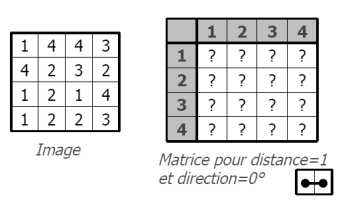
\includegraphics[width=0.65\textwidth]{Figures/cooc} % Include the image .png
	\caption{Classification des méthodes d’extraction de forme.}
\end{figure}

On parcours l'image et pour chaque couple de pixels formé avec la distance et la direction donn´ees, on incrémente la matrice des cooccurrences de 1. Alors la matrice de cooccurrence (non normalis´ee) est:

\begin{figure}[H]
	\label{fig:cooc_nn}
	\centering
	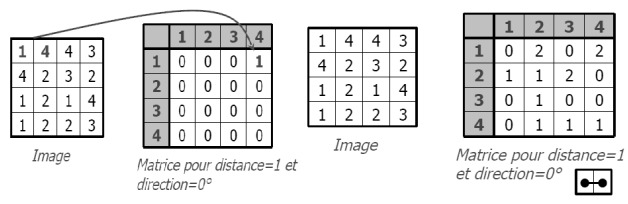
\includegraphics[width=0.8\textwidth]{Figures/cooc_non_norm} % Include the image .png
	\caption{Classification des méthodes d’extraction de forme.}
\end{figure}

Le 2 de la matrice de cooccurrence (ligne 1 et colonne 4) signifie que l’on trouve deux fois un pixel de valeur 1 de distance 1 et de direction
0 d’un pixel de valeur 4.

A partir de cette matrice de cooccurrence, il est possible de définir plusieurs descripteurs (Mesures de Haralick), tels que ceux répertoriés dans cette table:

\begin{table}[H]
	\centering
	\begin{tabular}{|{c}|l{c}|l|}
		
		\hline
		\textbf{ Mesure} & \textbf{  Formulation} \\
		\hline
		Uniformité/Energie & $E = \sum_{i=0}^{n}\sum_{j=0}^{n} P_{d,\theta}(i, j) $     \\
		\hline
		Entropie & $En = -\sum_{i=0}^{n}\sum_{j=0}^{n} P_{d,\theta}(i, j) \log_2 (P_{d,\theta}(i, j)) $    \\
		\hline
		Contraste & $ C = \sum_{i=0}^{n}\sum_{j=0}^{n} P_{d,\theta}(i, j) (i-j)^2 $ \\
		\hline
	Moment inverse de différence & $ M = \frac{1}{1+(i-j)^2} \sum_{i=0}^{n}\sum_{j=0}^{n} P_{d,\theta}(i, j)  $
	
	\end{tabular}
\caption{Mesure de Haralick}
\end{table}
 
 
\subsubsection{Transformée en ondelettes}
 Le terme " ondelette " en anglais (wavelet) a été utilisé pour la première fois en 1984 par J. Morlet et A. Grossmann pour résoudre des problèmes de traitement des signaux pour la prospection pétrolière.
 
 Une ondelette est une fonction à la base de la décomposition en ondelettes, décomposition similaire à la transformée de Fourier à court terme. La transformée en ondelettes consiste à décomposer un signal par une cascade de filtres pour générer une famille d’ondelettes appelées les ondelettes filles, obtenues par la translation et la dilatation d’une fonction mère. Chaque ondelette à une certaine fréquence pendant un temps limité, de la même façon que les notes de musique. La formule suivante présente une ondelette fille :
\begin{center}
	\begin{equation}
		$ \psi_{a,b}(t) = \frac{1}{\sqrt{a}} \psi(\frac{t-b}{a}) $
	\end{equation}
\end{center}
  

Le paramètre a est le facteur d’échelle, il détermine la dilatation de l'atome de base (ondelette fille). Le paramètre b est le facteur de translation, il permet de translater l'atome de base à gauche ou à droite. Le paramètre $ \frac{1}{\sqrt{a}} $ est un facteur de normalisation à travers les différentes échelles.\\

La transformée en ondelettes est un outil mathématique récent qui décompose un signal en fréquences en conservant une localisation spatiale. Le signal de départ est projeté sur un ensemble de fonctions de base qui varient en fréquence et en espace. Ces fonctions de base s’adaptent aux fréquences du signal à analyser. Cette transformation permet donc d’avoir une localisation en temps et en fréquence du signal analysé. La transformation en ondelettes continue est définie par :
		 \begin{center}
		 	\begin{equation}
		 	$ \tilde{f}(a,b) = \underset{-\infty }{\overset{+\infty }{\int }}f\left(t\right) \psi_{a,b}^*(t) dt   $
		 	\end{equation}
		 \end{center}
Dans cette équation, $ \psi_{a,b}^*(t) $ est la fonction de base d’ondelette. L’étoile «*» représente le complexe conjugué.

À partir de la transformée en ondelettes on peut extraire des attributs de différents types et à différents niveaux de résolution. L'image d'approximation donne des informations sur les régions qui composent l'image, d'une résolution fine à une résolution grossière. Les images de
détails donnent des informations horizontales, verticales et diagonales sur l'image [13]. Donc les ondelettes permettent de caractériser la texture en décrivant les primitives et les règles d'arrangement qui les relient.


\subsubsection{Les filtres de Gabor}

Les filtres de Gabor sont largement utilisés en indexation, pour la description de la texture.
Introduit par Gabor [Gabo46], ces filtres ont été largement utilisés [Chaw16] à la fois comme fonctions de décomposition en ondelettes et comme outils d'analyse texturale [Anda10]. Ces filtres peuvent prendre en compte l'orientation, l'échelle et la localisation des frontières, qui peuvent être
utilisés pour caractériser la texture. Les filtres de Gabor sont des filtres passe bande, leur forme générale résulte de la multiplication d’une fonction de forme d'enveloppe gaussienne avec une fonction sinusoïdale complexe.

Les filtres de Gabor sont largement utilisés aujourd’hui pour modéliser la réponse du système visuel humain. En effet, ce dernier décompose les images texturées en un nombre important d'images filtrées dont chacune contient les variations d'intensité à travers une bande de fréquence et une orientation bien déterminées [Partio 02]. En effet, Marcelaje [Marcelaje 80] a montré que les cellules du cortex humain pouvaient être modélisées par des fonctions de Gabor à une dimension. Cette décomposition a été utilisée par Manjunath [Manjunathi 96] pour des indexations par les textures.

Les filtres de Gabor permettent une bonne résolution spatiale à haute fréquence et une bonne résolution harmonique sans grande précision spatiale à basse fréquence [Merc01]. Sommairement, les paramètres de texture sont déterminés en calculant la moyenne et l’écart type des niveaux de gris de l’image filtrée par le filtre de Gabor. En fait, ce n’est pas une seule valeur de moyenne et d’écart type qui sera calculée, mais plutôt un ensemble de valeurs égal au nombre d’échelles multiplié par le nombre
d’orientations utilisées. Nous aurons donc ce qui est parfois appelé la banque de filtre de Gabor. Mathématiquement, toutes les valeurs des moyennes et d’écarts type calculées seront regroupées dans un seul vecteur descripteur. \\

Un filtre de Gabor 2D est le produit d'une gaussienne elliptique dans toute rotation et un exponentiel complexe représentant une onde plane sinusoïdale. Nous rappelons que, dans le domaine spatial, la fonction de Gabor bidimensionnelle est une somme de deux fonctions sinusoïdales, l'une paire et réelle, l'autre impaire et imaginaire, modulée par une enveloppe gaussienne. Une fonction Gabor 2D $g(x, y)$ et sa transformée de Fourier $G(u, v)$ s'écrivent comme suit [Manj96]:


 
\begin{center}
	 \begin{equation}
	
	$ g(x, y) = \frac{1}{2\pi \sigma_x \sigma_y} \exp\left[-\frac{1}{2} (\frac{x^2}{\sigma_x^2} + \frac{y^2}{\sigma_y^2}) + 2\pi j W_x\right]$
	\end{equation}
\end{center}

  \begin{center}
 	\begin{equation}
 	
 	$ g_{mn}(x, y) = a^{-m} \exp\left[-\frac{1}{2} (\frac{(u-W)^2}{\sigma_u^2} + \frac{v^2}{\sigma_v^2})\right] $
 	\end{equation}
 \end{center}

 avec : $\sigma_u = \frac{1}{2\pi \sigma_x } $ et  $ \sigma_v = \frac{1}{2\pi  \sigma_y} $. \\
 
 Un ensemble de fonctions similaires peut être générées à partir de la dilatation et la rotation de la fonction Gabor $g(x, y)$ :
 
 \begin{center}
 	\begin{equation}
 	
 	$ G(u, v) = a^{-m} g(x', y')
 	\end{equation}
 \end{center}
 
 où : $a \ge 1 $, $x' = a^{-m} ( x \cos(\theta) + y \sin(\theta) )$,  $y' = a^{-m} ( -x \cos(\theta) + y \sin(\theta) )$ , $\theta = \frac{n\pi}{K}$ et $m,n$ sont des entiers et indiquent l'échelle et l’orientation des ondelettes respectivement avec $m = 0,1,..., M-1 $,  $n=0,1,..., N-1$, et $K$ est le nombre d'orientations. Le facteur d’échelle $ a^{-m} $ vise à assurer que l'énergie est indépendante de $m$. Les paramètres $W$ et $\theta$ représentent la fréquence et l'orientation du signal sinusoïdal et constituent le paramètre de l’espace du filtre de Gabor.\\

\begin{figure}[H]
	\label{fig:gaborFig}
	\centering
	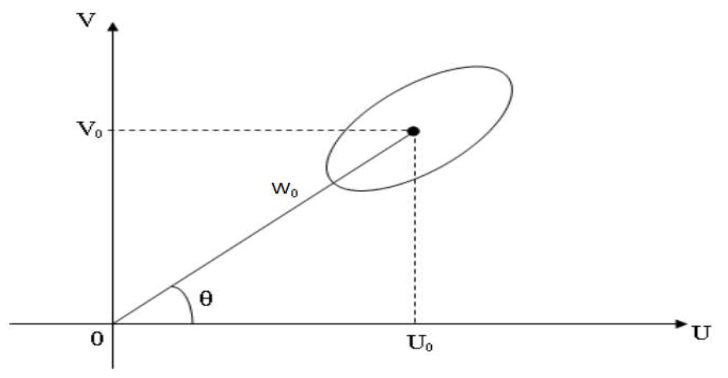
\includegraphics[width=0.65\textwidth]{Figures/gaborFig} % Include the image .png
	
	\caption{Contour à mi-niveau de la réponse en fréquence d’un filtre de Gabor 2D de fréquence centrale $W_0$ et d’orientation $\theta$.}
	
\end{figure}

L'utilisation des filtres de Gabor permet d'extraire de l'image considérée des informations pertinentes, à la fois en espace et en fréquence. Ils peuvent capturer le spectre de fréquence d'une image, en amplitude zt en phase. Ces filtres sont toujours utilisés par bancs dans lesquels chacun des filtres est réglé à une orientation et une fréquence précise. Les recherches conduites dans la littérature montrent que les fonctions de Gabor simulent de manière convenable le système visuel humain en reconnaissance des textures; le système visuel étant considéré comme un ensemble de canaux de filtrage dans le domaine fréquentiel.
 \begin{figure}[H]
 	\label{fig:gabor49}
 	\centering
 	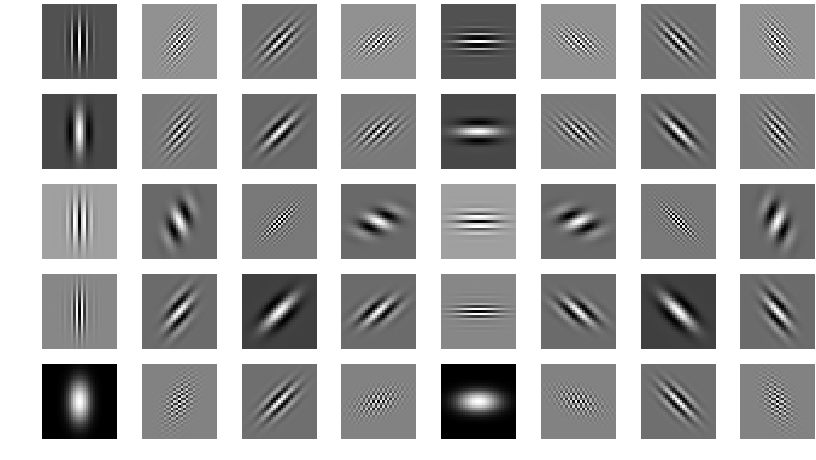
\includegraphics[width=0.65\textwidth]{Figures/gabor49} % Include the image .png
 	
 	\caption{Exemple du module des filtres de Gabor dans le domaine spatial.}
 	
 \end{figure}
 
 
\subsubsection{Conclusion}

Les attributs texturaux sont des attributs très importants pour la description de l'image et la
reconnaissance des objets, cependant elles ne suffisent pas pour une bonne représentation du
contenu de l'image, un autre attribut essentiel est la forme.
Dans la suite nous allons introduire cet attribut et les différentes approches utilisées pour
l'extraire.


Une grande partie de la recherche sur la description des textures s'est concentrée sur les techniques multi-échelles, notamment la transformée en ondelettes [Laws 80], [Mallat 99], [Strang 97]. Cette description a été avancée grâce à l'exploitation de modèles statistiques multi-échelles markoviens. Un framework multirésolution est le cadre le plus naturel pour la description de la texture. Une technique multi-échelles commune est la Transformée en Ondelettes Discrètes (DWT).

Les textures se produisent dans les régions d'une image, et doivent être décrites principalement en analysant l'information sur l'intensité à la résolution appropriée. Toutes les textures n'apparaissent pas sur les mêmes gammes régionales, c'est pourquoi une approche qui varie la taille de la région d'intérêt est souhaitable. Les techniques multi-échelles fournissent une grande capacité de la description de la texture.

Les structures markoviennes ont également été utilisées avec succès pour l'identification et la modélisation des textures [Choi 01], [Crousse 98].

\subsection{Descripteur de forme}
Si l'être humain est particulièrement sensible à l'attribut de couleur pour distinguer les
objets, pour certains types d'ambiguïté cela n'est pas suffisant et l'on a besoin de l'attribut de forme. Au même titre que pour la texture, l’information de forme également appelée en anglais « Shape » est complémentaire de celle de la couleur. La forme est généralement une description très riche d’un objet. Elle permet de détecter un objet sur une image plutôt que l’image elle-même.\\

La forme est un descripteur très important dans l'indexation des images. Elle est utilisée pour décrire la structure géométrique générique du contenu visuel. Généralement, les descripteurs de formes se divisent en deux catégories: les méthodes régions s'appuient sur la forme entière et les autres sur le contour. On peut ensuite distinguer deux familles pour chacune de ces catégories, une famille qui considère les objets comme une seule partie, et celle qui décrit les objets en les considérant comme un assemblage de sous parties. Une segmentation des objets est généralement utilisée avant l’extraction des attributs.

\begin{figure}[H]
	\label{fig:forme}
	\centering
	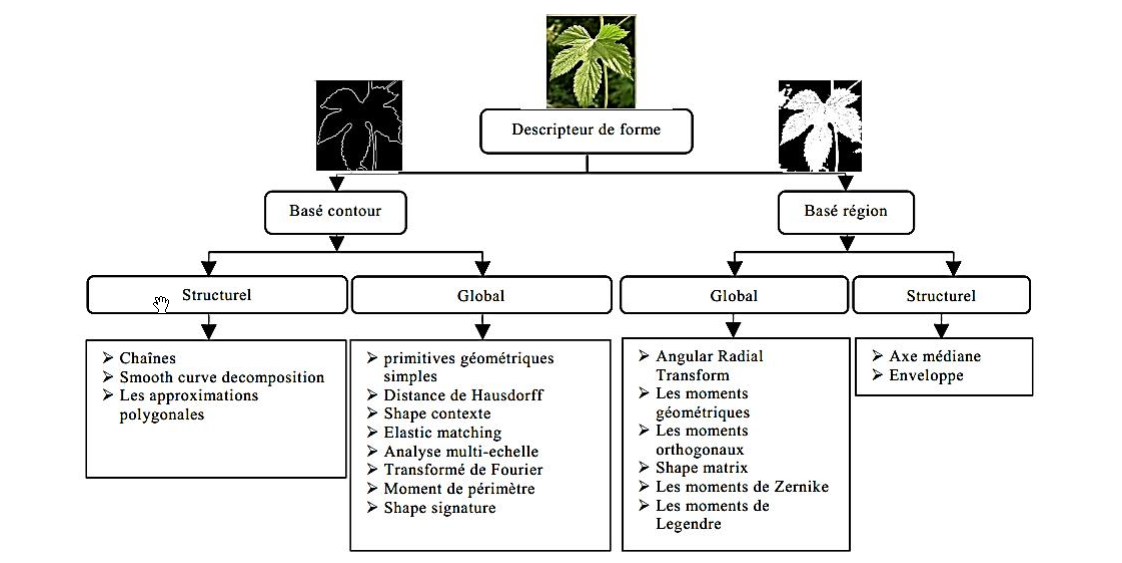
\includegraphics[width=0.65\textwidth]{Figures/forme} % Include the image .png
	
	\caption{Classification des méthodes d'extraction de forme.}
	
\end{figure}

Nous présentons dans ce qui suit quelques méthodes de description de la forme :

\subsection{Descripteurs de Fourier}
Les descripteurs de Fourier (DFs) font partie des descripteurs les plus populaires pour les applications de reconnaissance de forme et de recherche d’images. Ils ont souvent été utilisés par leur
simplicité et leurs bonnes performances en terme de reconnaissance [Zhan05] et facilitent l’étape
d’appariement. De plus, ils permettent de décrire la forme de l’objet à différents niveaux de détails.
Les DFs sont calculés à partir du contour des objets. Leur principe est de représenter le contour de
l’objet par un signal 1D, puis de le décomposer en séries de Fourier. Les DFs sont généralement
connus comme une famille de descripteurs car ils dépendent de la façon dont sont représentés les
objets sous forme de signaux.

\subsubsection{Moments géométriques}
Les moments géométriques [Sonk99] permettent de décrire une forme à l’aide de propriétés
statistiques. Ils représentent les propriétés spatiales de la distribution des pixels dans l’image.
La formule générale des moments géométriques est donnée par la relation suivante :

\begin{equation}
	$m_{p,q} = \sum_{x=0}^{M-1}\sum_{y=0}^{N-1} x^p y^q f(x, y) $   
	
\end{equation}

avec $p+q$ est l'ordre du moment. Le moment d’ordre $0 (m_{0,0})$  représente l’aire de la forme de l'objet, $f(x, y)$ : luminance du pixel (x, y), c’est-à-dire noir ou blanc en binaire.

Les moments géométriques sont très robustes et peu sensibles au bruit, préservation de l’information, facilement calculés et implémentés. Par contre, cette approche a des inconvénients comme la difficulté à corréler les moments avec la forme en elle-même, très sensible aux déformations et le temps de calcul de ces moments est très long.

\subsubsection{Moments orthogonaux}
Par opposition aux moments géométriques qui sont définis par rapport à une base quelconque $(x^p, y^q)$, les moments orthogonaux, comme leur nom l’indique, sont définis dans une base orthogonale, ce qui évite la redondance des informations portées par chacun des moments. Les deux types de moments orthogonaux les plus utilisés sont : les moments de Legendre et les moments de Zernik.

\subsubsection{Descripteurs de Fourier}
Les descripteurs de Fourier (DFs) font partie des descripteurs les plus populaires pour les applications de reconnaissance de forme et de recherche d’images. Ils ont souvent été utilisés par leur simplicité et leurs bonnes performances en terme de reconnaissance [Zhan05] et facilitent l'étape d'appariement. De plus, ils permettent de décrire la forme de l’objet à différents niveaux de détails.

Les DFs sont calculés à partir du contour des objets. Leur principe est de représenter le contour de l'objet par un signal 1D, puis de le décomposer en séries de Fourier. Les DFs sont généralement connus comme une famille de descripteurs car ils dépendent de la façon dont sont représentés les objets sous forme de signaux.

\subsubsection{Transformation ART}
Angular Radial Transform (ART) est un descripteur de forme robuste au changement d’échelle, à la translation et à la rotation et utilisé dans plusieurs travaux [AitZ14], [Chaw16]. Ce descripteur consiste à projeter l’objet à étudier sur une série de fonctions de base [Kim99]. Il a été
adopté par la norme MPEG-7. Il permet de décrire la forme d’une région de manière compacte et efficace, à partir de la distribution 2D des pixels de cette région. Formellement, ART est une transformation complexe unitaire définie sur un disque unité, qui consiste en une projection de
l’image sur des fonctions de bases, dans un repère polaire. De plus ART est une méthode basée sur les régions et traite la forme dans son ensemble et utilise l’information de tous les pixels de la région. Cette méthode mesure la distribution des pixels de la région et est peu affectée par le bruit et par les variations de formes.

Pour ces différentes raisons, nous nous sommes principalement intéressés aux méthodes d’analyses de formes basées régions, et plus précisément à la transformation ART dans notre travail.

%
% Les descripteurs basés sur le contour incluent les descripteurs de Fourier [Rui 98], [Zhang 05], et les chaînes de Freeman, qui ont été largement utilisés.
% 
%  Les descripteurs basés sur la région prennent en compte tous les pixels de la forme et les méthodes les plus courantes sont basées, sur la théorie des moments [Prokop 92], [Hu 62], [Jiang 91], [Taubin 92].
%   
%   Les moments invariants offrent une description robuste aux transformations affines, propriété appréciable pour les systèmes CBIR.
%
%Quelle que soit la méthode utilisée, il demeure important que certaines propriétés d'invariance soient vérifiées, notamment pour la translation, le changement d’échelle et la rotation, du fait que l’être humain corrige instinctivement les effets de ces transformations lors de la recherche d’un objet. Dans certaines applications, la robustesse à l’occultation peut également être souhaitée.
%
%Pour rechercher des formes similaires, des mesures de similarité entre des descripteurs sont définies pour déterminer la distance entre eux. Cependant, la comparaison n’est pas toujours simple et elle exige parfois des transformations. De plus, la dimension du descripteur est souvent élevée, ce qui augmente la complexité quand on cherche des objets similaires dans une grande collection.






\section{Mesure de similarité entre attributs}
La mesure de similarité est une étape fondamentale dans la recherche
d’images par le contenu. Elle compte sur la mesure de la ressemblance
visuelle entre une image requête et les images de la base. 

Les performances d'un CBIR dépendent largement de la mesure de similarité utilisée pour la comparaison des descripteurs des images. La mesure de similarité est aussi dépend des critères de la recherche mais également de la représentation des caractéristiques.

La mesure de similarité quantifiée la proximité des images dans l'espace des caractéristiques. Elle est souvent métrique, les images sont considérées ressemblantes si la distance est faible. La complexité de calcul d'une distance doit être raisonnable par ce que dans un système CBIR cette tâche s'exécute en temps réel ou pseudo réel. D'autres paramètres entrent en jeu telle la dimension de l'espace caractéristique, la taille de la base... La méthode naïve de recherche calcule la distance entre la requête et toutes les images de la base puis les ordonne selon leur score. Ceci par conséquent rend le temps de réponse proportionnel au
nombre d'images (O(N)). Les méthodes d'indexation du contenu permettent par ailleurs de réduire cette complexité comparée à la recherche séquentielle. Pour résumer, la mesure de similarité vérifie généralement les propriétés :

\begin{itemize}
	\item  \textbf{La perception} : Une faible distance dans l'espace de caractéristique indique deux images semblables.
	
	\item \textbf{Le calcul} : La mesure de distance se calcule rapidement pour une faible latence.
	
	\item \textbf{La scalabilité }: Le calcul de distance ne doit pas être affecté par une modification de taille de la base.
	
	\item \textbf{La robustesse} : La mesure devra être robuste aux changements des conditions d'acquisition d'image.
\end{itemize}


En mathématiques, on appelle distance sur un ensemble $E$ une application $d$ définie sur le produit $E^2 = E \times E$ et à valeurs dans l'ensemble $R^+$ des réels positifs:

\begin{figure}[H]
	\centering
	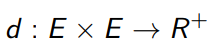
\includegraphics[width=0.2\textwidth]{Figures/distanceApp.png} % Include the image .png
\end{figure}

vérifiant les propriétés suivantes :

\begin{figure}[H]
	\centering
	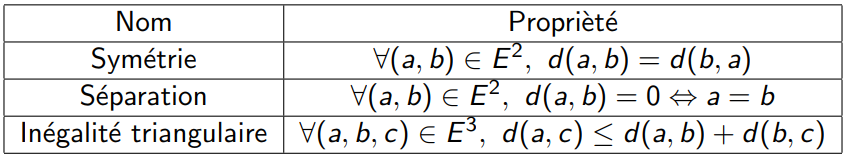
\includegraphics[width=0.8\textwidth]{Figures/distanceProp.png} % Include the image .png
\end{figure}

Un ensemble muni d'une distance est un espace métrique.\\


Nous citons ci-dessous les distances les plus utilisées pour comparer des images considérées comme vecteurs ou comme distributions statistiques.

\subsection{Distances de Minkowski}
La distance de Minkowski est une famille de distances vectorielles. Soit $I_1$ , $I_2$ deux vecteurs de caractéristiques, elle s'exprime par :

\begin{equation}
       $d_p(I_1, I_2) = \sum_{i=1}^{N} \sqrt[p]{\left|{I}_{1}(i)-{I}_{2}(i)\right|^p} $ 
\end{equation}

Où $p\geq 1$ est le facteur de Minkowski et $N$ la dimension de l’espace caractéristique. Les métriques de Minkowski sont simples d’utilisation, rapides à calculer, simples à implémenter, et représentent un bon compromis entre efficacité et performance, par contre leur calcul est réalisé en considérant que chaque composante du vecteur apporte la même contribution à la distance. Pour cette famille de distances, plus le paramètre $p$ augmente, plus la distance $d_p$ aura tendance à favoriser les grandes différences entre coordonnées.

On distingue:
\begin{table}[H]
	\begin{tabular}{|c|c|c|}
		\hline
		\textbf{Distance} & \textbf{Caractéristiques}\\
		\hline
		\makecell{Manhatttan : \\ $d_1(I_1, I_2) = \sum_{i=1}^{N} \left|{I}_{1}(i)-{I}_{2}(i)\right| $ } & \makecell{Cette distance est plus convenable pour mesurer \\ la similarité entre les données multivariées, elle est\\ moins sensible au bruit coloré que \\la distance euclidienne. }   \\
		\hline
		
		
		\makecell{Euclidienne :\\ $d_2(I_1, I_2) = \sum_{i=1}^{N} \sqrt{\left|{I}_{1}(i)-{I}_{2}(i)\right|^2} $}  & \makecell{C’est la distance la plus fréquemment utilisée grâce \\à ses propriétés géométriques intéressantes. Cette distance \\à tendance à donner plus d’importance aux plus grandes \\différences sur une variable simple. Le contour de la\\ même distance (Euclidienne) à partir d’un point donnée\\ à une forme sphérique (cercle en deux dimensions).}   \\
		\hline
		
		\makecell{Chebychev :\\ $d_{\infty}(I_1, I_2) = \max_{i=1}^N  \left|{I}_{1}(i)-{I}_{2}(i)\right|} $}  & \makecell{La distance de Chebychev est adaptée aux données\\ de grande dimension, elle est souvent employée dans \\les applications où la vitesse d’exécution est importante.\\ Cette distance examine la différence absolue entre les différents\\ pairs des vecteurs, elle est considérée comme une approximation\\ de la distance Euclidienne mais avec moins de calcul.} \\   
		\hline
		
	
	\end{tabular}
	\caption{Les distances de Minkowski}
\end{table}

\subsection{Distance quadratique}
La distance de Minkowski traite les éléments du vecteur de
caractéristique d’une manière équitable. La distance quadratique en
revanche favorise les éléments les plus ressemblants. Les propriétés de cette distance la rendraient proche de la perception humaine de la couleur, ce qui en fait une métrique attractive pour les systèmes de Recherche d’images couleur par le contenu [16]. Sa formule générale est donnée par :

\begin{figure}[H]
	\centering
	\begin{equation}
	$d_q(I_1, I_2) = \sqrt{(I_1 - I_2)^T A (I_1 - I_2)} $
	\end{equation}
\end{figure}

Ou $A = (a_{ij}) $est la matrice de similarité. $a_{ij}$ représente la distance entre deux éléments des vecteurs $I_1$ et $I_2$, elle est définie par :

\begin{figure}[H]
	\centering
	\begin{equation}
	$a_{ij} = 1 - \frac{a_{ij}}{\max a_{ij}}$
	\end{equation}
\end{figure}

\subsection{Distance de Swain}
Cette mesure est l'une des premières distances utilisée dans la recherche d'image par le contenu, si les images d’une base des images sont indexées par des histogrammes, les distances géométriques s’appliquent. Cependant, il est possible de définir des mesures de similarité propres à cette représentation. Ainsi, l’intersection d’histogrammes est l’une des premières distances utilisée dans les systèmes CBIR [Swain91].Elle permet de comparer deux histogrammes normalisés $H_1$ et $H_2$ . La distance de Swain s’exprime ainsi :

\begin{figure}[H]
	\centering
	\begin{equation}
	$d_2(H_1, H_2) = 1- \frac{\sum_{i=1}^{N} \min(H_1(i),  H_2(i))}{\sum_{i=1}^{N}  H_2(i)}  $
	\end{equation}
\end{figure}

Il existe d’autres distances dans la littérature qui ne sont pas abordées dans ce mémoire.
\subsection{Conclusion}
Ce chapitre a fait l’état de l’art sans exhaustivité des différents descripteurs des attributs visuels pouvant être utilisés pour la recherche d’images par le contenu ainsi que les approches
correspondantes. Aussi, nous avons dressé une liste des types de descripteurs et les mesures de similarités avec leurs avantages et leurs inconvénients. Le chapitre suivant se focalisera sur notre solution détaillée, le schéma de CBIR, les techniques d’extraction de descripteur. Le choix d’un meilleur descripteur et d’une mesure de similarité promet une bonne pertinence d’un système CBIR.